\subsubsection{Intervención en la estimación de posición del robot}

Mencionamos anteriormente que el payload de los códigos QR contienen las coordenadas en el eje $X$e $Y$ en donde se encuentra el QR en el mapa. Al medir la distancia hacia el código lo que estamos haciendo es sumarle precisión a la determinación de la ubicación del robot. Entonces si tomamos como ejemplo ideal a una fotografía donde el código QR se encuentra perfectamente centrado, significa que el robot no presenta desplazamiento alguno el eje $X$.

\begin{figure}[H]
   \centering
   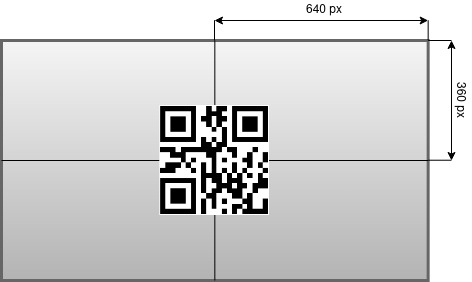
\includegraphics[width=0.7\linewidth]{images/ejemplo_foto_centro.jpg}
   \caption{Ejemplo de una fotografía con el código QR centrado}
   \label{fig:ejemplo_foto_centro}
\end{figure}

Entonces si nos basamos en la Figura \ref{fig:ejemplo_foto_centro} para determinar la posición del robot, obtenemos una posición mas precisa ya que si durante el procesamiento de la fotografía verificamos que el código QR se encuentra desplazado hacía la derecha, el robot va a estar desplazado hacía la izquierda sobre el eje $X$. Y si también el código QR detectado es de mayor dimensión en la imagen, el robot se encuentra posicionado más cerca del código QR.

Además cómo se mencionó mas arriba, el contenido del payload incluye las coordenadas en donde se encuentra el código dentro del plano. Entonces si tenemos el ejemplo donde un robot posicionado en la coordenada $(4,2)$ desea llegar a la coordenada $(4,0)$ donde se encuentra ubicado un código QR con las coordenadas descritas, nos encontramos en la situación en la que, por su posición actual, le es imposible al robot reconocer el código QR por la gran distancia que existe entre él y la cámara del robot, por lo tanto estimamos que el robot mientras realiza desplazamientos entre celda y celda siempre va a terminar posicionado al centro de ella.

\begin{figure}[H]
   \centering
   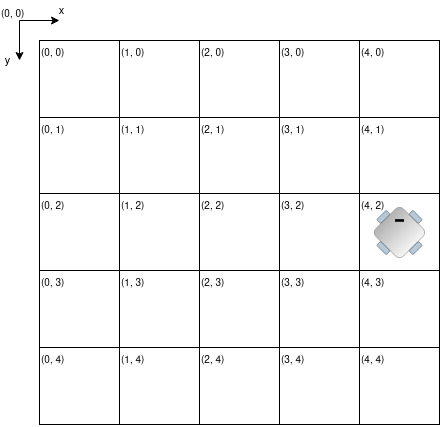
\includegraphics[width=0.5\linewidth]{images/robot_posicion_0.jpg}
   \caption{Robot posicionado en la coordenada $(4,2)$}
   \label{fig:robot_posicion_0}
\end{figure}

Ahora si el robot se encuentra llegando a su destino, la coordenada $(4,0)$ y se encuentra dentro del rango de distancia de reconocimiento de códigos QR, va a calcular la distancia tanto en el eje $Y$ como en el $X$ y sumarla al payload del código QR para después poder reportar esa coordenada. Entonces en ese momento, así como muestra la figura \ref{fig:robot_posicion_1} el robot en realidad se encuentra ubicado en la coordenada $(4.2,0.5)$ y no el centro de la celda como uno supone cuando no tiene el reporte de su ubicación en todo momento.

\begin{figure}[H]
   \centering
   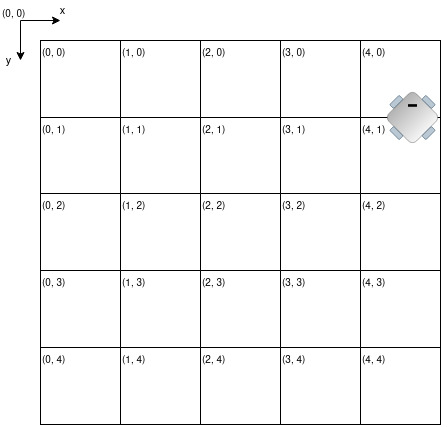
\includegraphics[width=0.5\linewidth]{images/robot_posicion_1.jpg}
   \caption{Robot posicionado en la coordenada $(4.2,0.5)$}
   \label{fig:robot_posicion_1}
\end{figure}

La siguiente imagen \ref{fig:qrcamararobot} muestra cómo es una fotografía captada en movimiento por el robot y la lectura que hace del payload, cómo se puede observar es una imagen bastante nítida y con buen enfoque lo que permite que el procesamiento de la misma se realice con mayor precisión.

\begin{figure}[H]
   \centering
   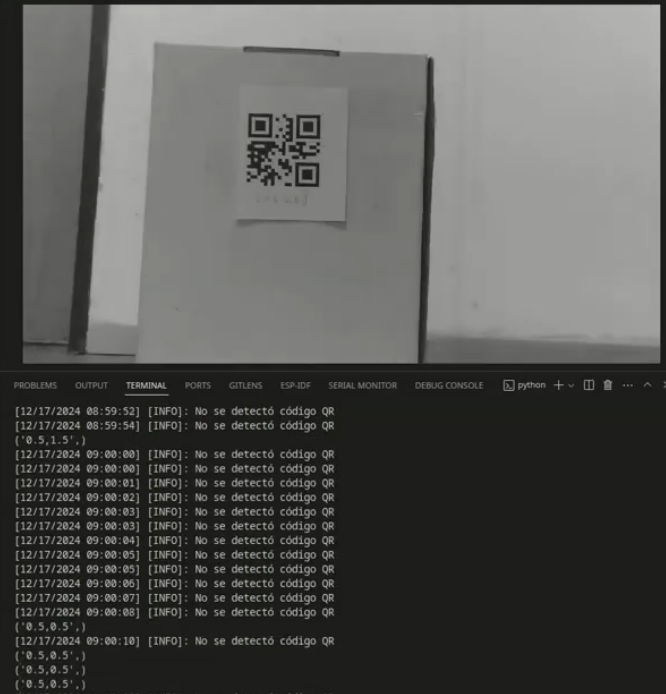
\includegraphics[width=0.7\linewidth]{images/qr.png}
   \caption{Imagen obtenida por el robot en movimiento}
   \label{fig:qrcamararobot}
\end{figure}